\chapter{\texorpdfstring{S/T-Systems}{S/T-Systems}}
\label{ch:15}
\lecturemeta{Lezione 15 \quad\textbullet\quad 2026-07-03 \quad\textbullet\quad Roberto Bruni}{Petri nets · Esparza, \emph{Free Choice Petri Nets} (optional)}

Le proprietà comportamentali (boundedness, liveness) sono costose da verificare in generale, perché richiedono di esplorare gli stati. L'idea di questa lezione è: \textbf{restringere la classe di reti} a due famiglie particolarmente "pulite" e, per esse, dare \textbf{caratterizzazioni puramente strutturali} di quelle proprietà — controllabili guardando solo la forma del grafo, senza token game. Le due famiglie sono gli \textbf{S-system} (che vietano la sincronizzazione) e i \textbf{T-system} (che vietano la scelta), e sono l'una il \textbf{duale} dell'altra.

Il problema che vogliamo evitare è l'\textbf{interferenza tra conflitti e sincronizzazione}: in una rete generale due transizioni possono passare dall'essere indipendenti all'essere in conflitto a seconda di cosa scatta prima, e questo rende l'analisi difficile. Restringendo la struttura, questa interferenza scompare.

\section{\texorpdfstring{Le due classi: S-net e T-net}{Le due classi: S-net e T-net}}

La distinzione è sorprendentemente semplice e riguarda quanti archi hanno i nodi.

\begin{boxdefinition}{S-net e T-net}
\begin{itemize}
\item Una rete è un \textbf{S-net} se \textbf{ogni transizione ha esattamente un input place e un output place}:
\end{itemize}

\[
\forall t.\; |\bullet t| = 1 = |t\bullet|
\]

(La S viene da \emph{Stellen}, "place" in tedesco.) Una transizione così \textbf{non può sincronizzare} (non aspetta più input) né \textbf{spezzare} (non produce più output): la sincronizzazione è \textbf{vietata}. - Una rete è un \textbf{T-net} se \textbf{ogni place ha esattamente una input transition e una output transition}:

\[
\forall p.\; |\bullet p| = 1 = |p\bullet|
\]

Un place così \textbf{non può essere conteso} da più transizioni: la \textbf{scelta/conflitto è vietata}. I T-net sono \textbf{concorrenti ma deterministici}.
\end{boxdefinition}

\begin{figure}[!htb]
\centering
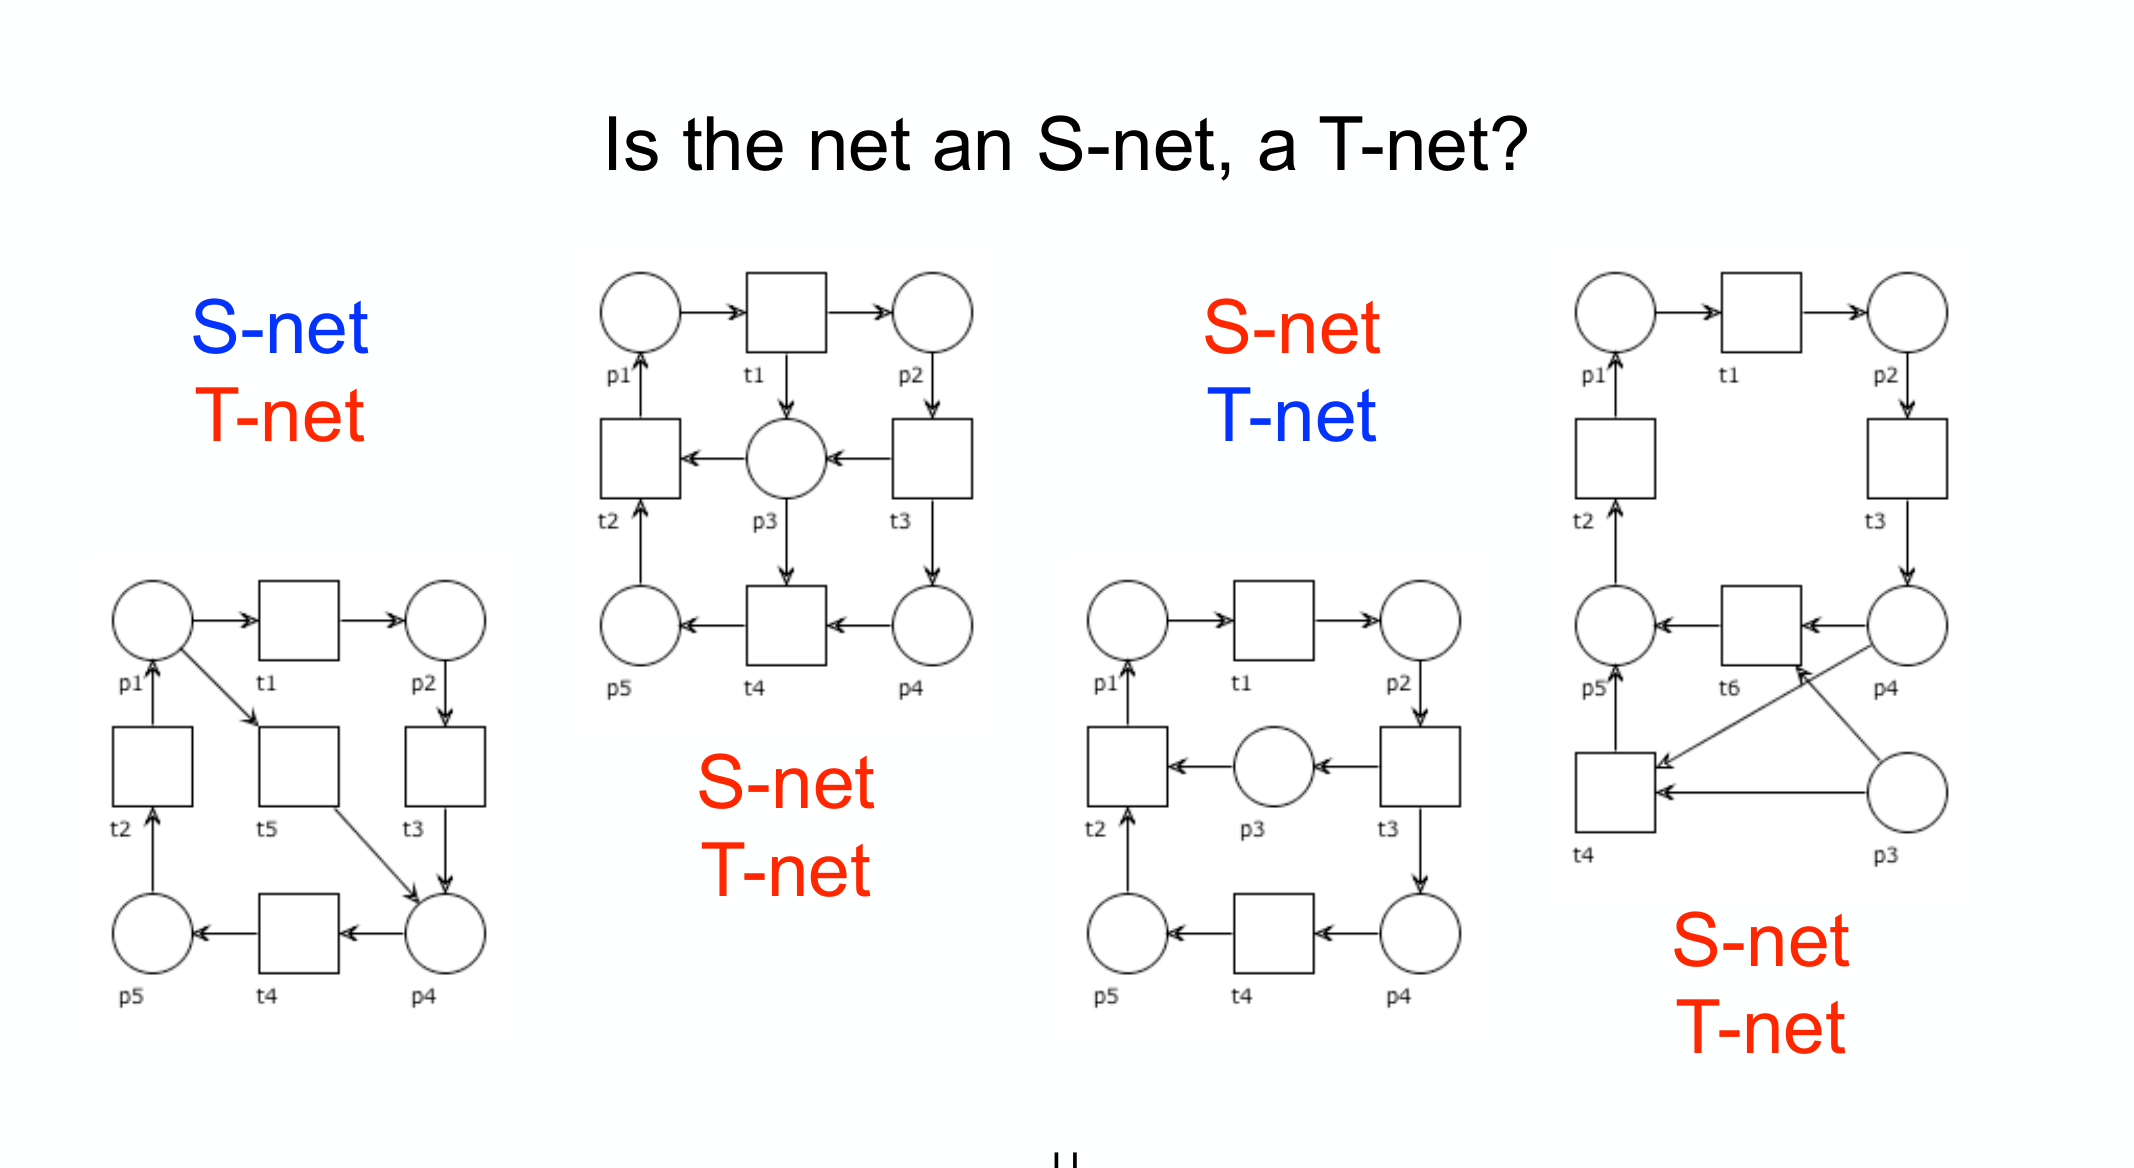
\includegraphics[width=0.74\linewidth,height=0.34\textheight,keepaspectratio]{images/15-st-systems_p10_s-net-t-net.png}
\caption{Classificare S-net e T-net. Si guarda ogni transizione (per S-net: una freccia in, una out) e ogni place (per T-net: una in, una out). Le due proprietà sono indipendenti: una rete può essere solo S, solo T, entrambe, o nessuna delle due.}
\end{figure}

Un \textbf{S-system} (risp. \textbf{T-system}) è semplicemente un net system $(N, M_0)$ dove $N$ è un S-net (risp. T-net). La bellezza è che per queste classi tutto diventa facile — al punto che, come vedremo, valgono due "take-home message" fortissimi sui workflow net.

\section{\texorpdfstring{S-systems: la conservazione dei token}{S-systems: la conservazione dei token}}

Poiché in un S-net ogni transizione toglie \textbf{esattamente un} token da un place e ne mette \textbf{esattamente uno} in un altro, il numero totale di token nella rete non cambia mai. È l'analogo di una legge di conservazione.

\begin{boxtheorem}{Proprietà fondamentale degli S-system}
Il \textbf{numero totale di token} è invariante. Detto $M(P) = \sum_{p \in P} M(p)$ il conteggio totale, per ogni marcatura raggiungibile $M \in [M_0\rangle$ vale:

\[
M(P) = M_0(P)
\]

\emph{Perché:} ogni scatto fa

\[
M'(P) = M(P) - |\bullet t| + |t\bullet| = M(P) - 1 + 1 = M(P)
\]
\end{boxtheorem}

Da questo discendono subito diverse conseguenze, tutte immediate.

\begin{boxnote}{Conseguenze immediate per gli S-system}
\begin{itemize}
\item \textbf{Sempre bounded}: da
\end{itemize}

\[
M(p) \le M(P) = M_0(P)
\]

nessun place può superare $M_0(P)$ token. Un S-system è k-bounded con $k = M_0(P)$. - \textbf{Test di raggiungibilità gratis}: se $M(P) \ne M_0(P)$, allora $M$ \textbf{non è raggiungibile}. (Es. se parto con 6 token in totale, una marcatura con 7 token è impossibile.) - \textbf{S-invariant uniformi}: gli unici S-invariant di un S-net connesso sono i vettori costanti $I = [k, k, \dots, k]$ — coerente con "ogni token vale uguale, la somma si conserva".
\end{boxnote}

E la liveness? Ha una caratterizzazione \textbf{puramente strutturale}, il primo dei risultati che cercavamo.

\begin{boxtheorem}{Liveness degli S-system}
Un S-system $(N, M_0)$ è \textbf{live} $\iff$

\[
N \text{ è strongly connected} \quad \text{e} \quad M_0(P) \ge 1
\]

\emph{Intuizione ($\Leftarrow$):} con un token in giro e strong connectedness, per abilitare una qualsiasi transizione $t$ basta \textbf{spostare il token fino a lei} lungo un cammino (che esiste, per la strong connectedness); poiché ogni transizione dell'S-net sposta solo il token, la si può portare dove serve.
\end{boxtheorem}

Combinando conservazione e strong connectedness si ottiene anche una caratterizzazione \textbf{esatta della raggiungibilità} — cosa rarissima, dato che in generale è EXPSPACE-hard.

\begin{boxtheorem}{Raggiungibilità negli S-system live}
In un S-system \textbf{live} (quindi strongly connected), una marcatura $M$ è \textbf{raggiungibile} $\iff$

\[
M(P) = M_0(P)
\]

Cioè: basta contare i token. Se $M$ ha lo stesso numero totale di token di $M_0$, allora è raggiungibile (li si sposta uno per volta nei place giusti sfruttando i cammini); altrimenti no.
\end{boxtheorem}

\begin{boxtip}{Take-home message (S-net)}
\textbf{Ogni workflow net che sia un S-net è safe e sound.} La catena: un WF net S-net ha $N^\star$ ancora S-net $\rightarrow$ è bounded; è strongly connected (perché è un WF net con reset) e $M_0(P)=1$ $\rightarrow$ $N^\star$ è live; live + bounded $\iff$ $N$ sound (\hyperref[ch:12]{12 — Soundness}). Il singolo token che scorre garantisce automaticamente la correttezza.
\end{boxtip}

\section{\texorpdfstring{T-systems: la conservazione sui circuiti}{T-systems: la conservazione sui circuiti}}

Passiamo al duale. In un T-net non c'è conservazione del numero \emph{totale} di token (una transizione può avere più input e output place). Ma c'è una conservazione più sottile, sui \textbf{circuiti}.

Ricordiamo che un \textbf{circuito} è un cammino ciclico $\gamma$; scriviamo $M(\gamma)$ per il numero di token nei place del circuito, e diciamo che $\gamma$ è \textbf{marcato} se $M(\gamma) > 0$.

\begin{boxtheorem}{Proprietà fondamentale dei T-system}
Il \textbf{conteggio dei token di ogni circuito} è invariante: per ogni circuito $\gamma$ e ogni $M \in [M_0\rangle$:

\[
M(\gamma) = M_0(\gamma)
\]

\emph{Perché:} prendi una transizione $t$. In un T-net, o $t$ non tocca il circuito $\gamma$ (allora non ne cambia i token), oppure lo tocca — ma allora consuma da \textbf{esattamente un} place di $\gamma$ e produce in \textbf{esattamente un} place di $\gamma$ (per la struttura 1-in-1-out dei place), quindi il conteggio resta invariato. In ogni caso $M(\gamma)$ non cambia.
\end{boxtheorem}

\begin{figure}[!htb]
\centering
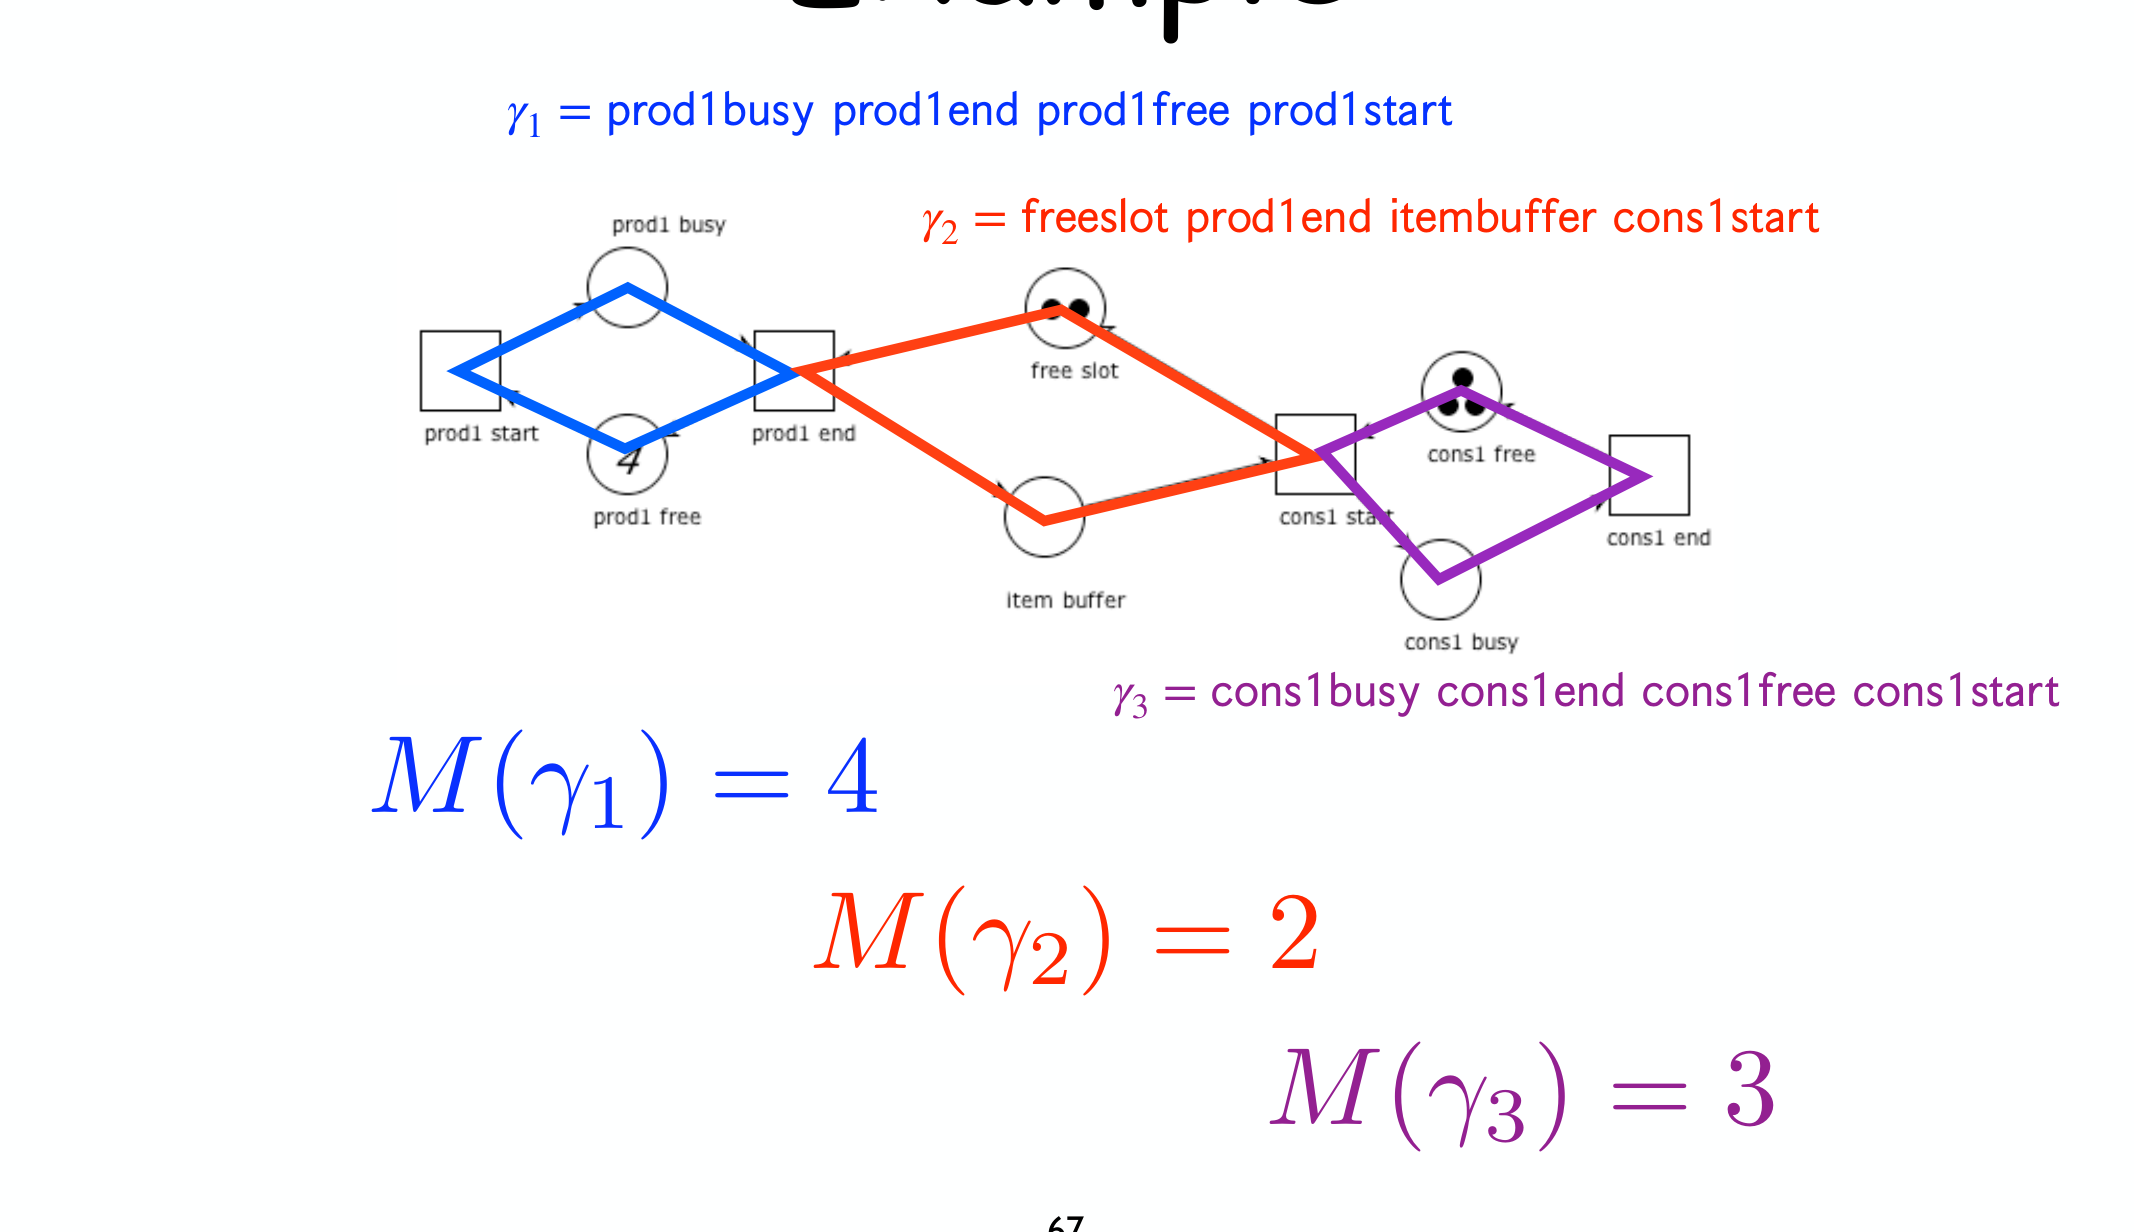
\includegraphics[width=0.74\linewidth,height=0.34\textheight,keepaspectratio]{images/15-st-systems_p66_circuits.png}
\caption{I circuiti di un T-system e i loro conteggi. Ogni circuito è come un "anello" con un numero fisso di token che ci girano dentro: $M(\gamma_1)=4$, $M(\gamma_2)=2$, $M(\gamma_3)=3$ resteranno tali per sempre. È l'analogo, sui circuiti, della conservazione totale degli S-system.}
\end{figure}

Anche qui le conseguenze sono immediate e speculari a quelle degli S-system.

\begin{boxnote}{Conseguenze per i T-system}
\begin{itemize}
\item \textbf{Test di raggiungibilità}: se $M(\gamma) \ne M_0(\gamma)$ per qualche circuito $\gamma$, allora $M$ \textbf{non è raggiungibile}.
\item \textbf{Boundedness da strong connectedness}: se un T-system è strongly connected, è \textbf{bounded} (ogni place sta in qualche circuito, il cui conteggio è limitato). È \textbf{safe} se $M_0(P)=1$ (o più in generale se ogni circuito ha $\le 1$ token).
\item \textbf{T-invariant uniformi}: gli unici T-invariant di un T-net connesso sono i vettori costanti $J = [k, \dots, k]$ (duale del risultato sugli S-net).
\end{itemize}
\end{boxnote}

\begin{figure}[!htb]
\centering
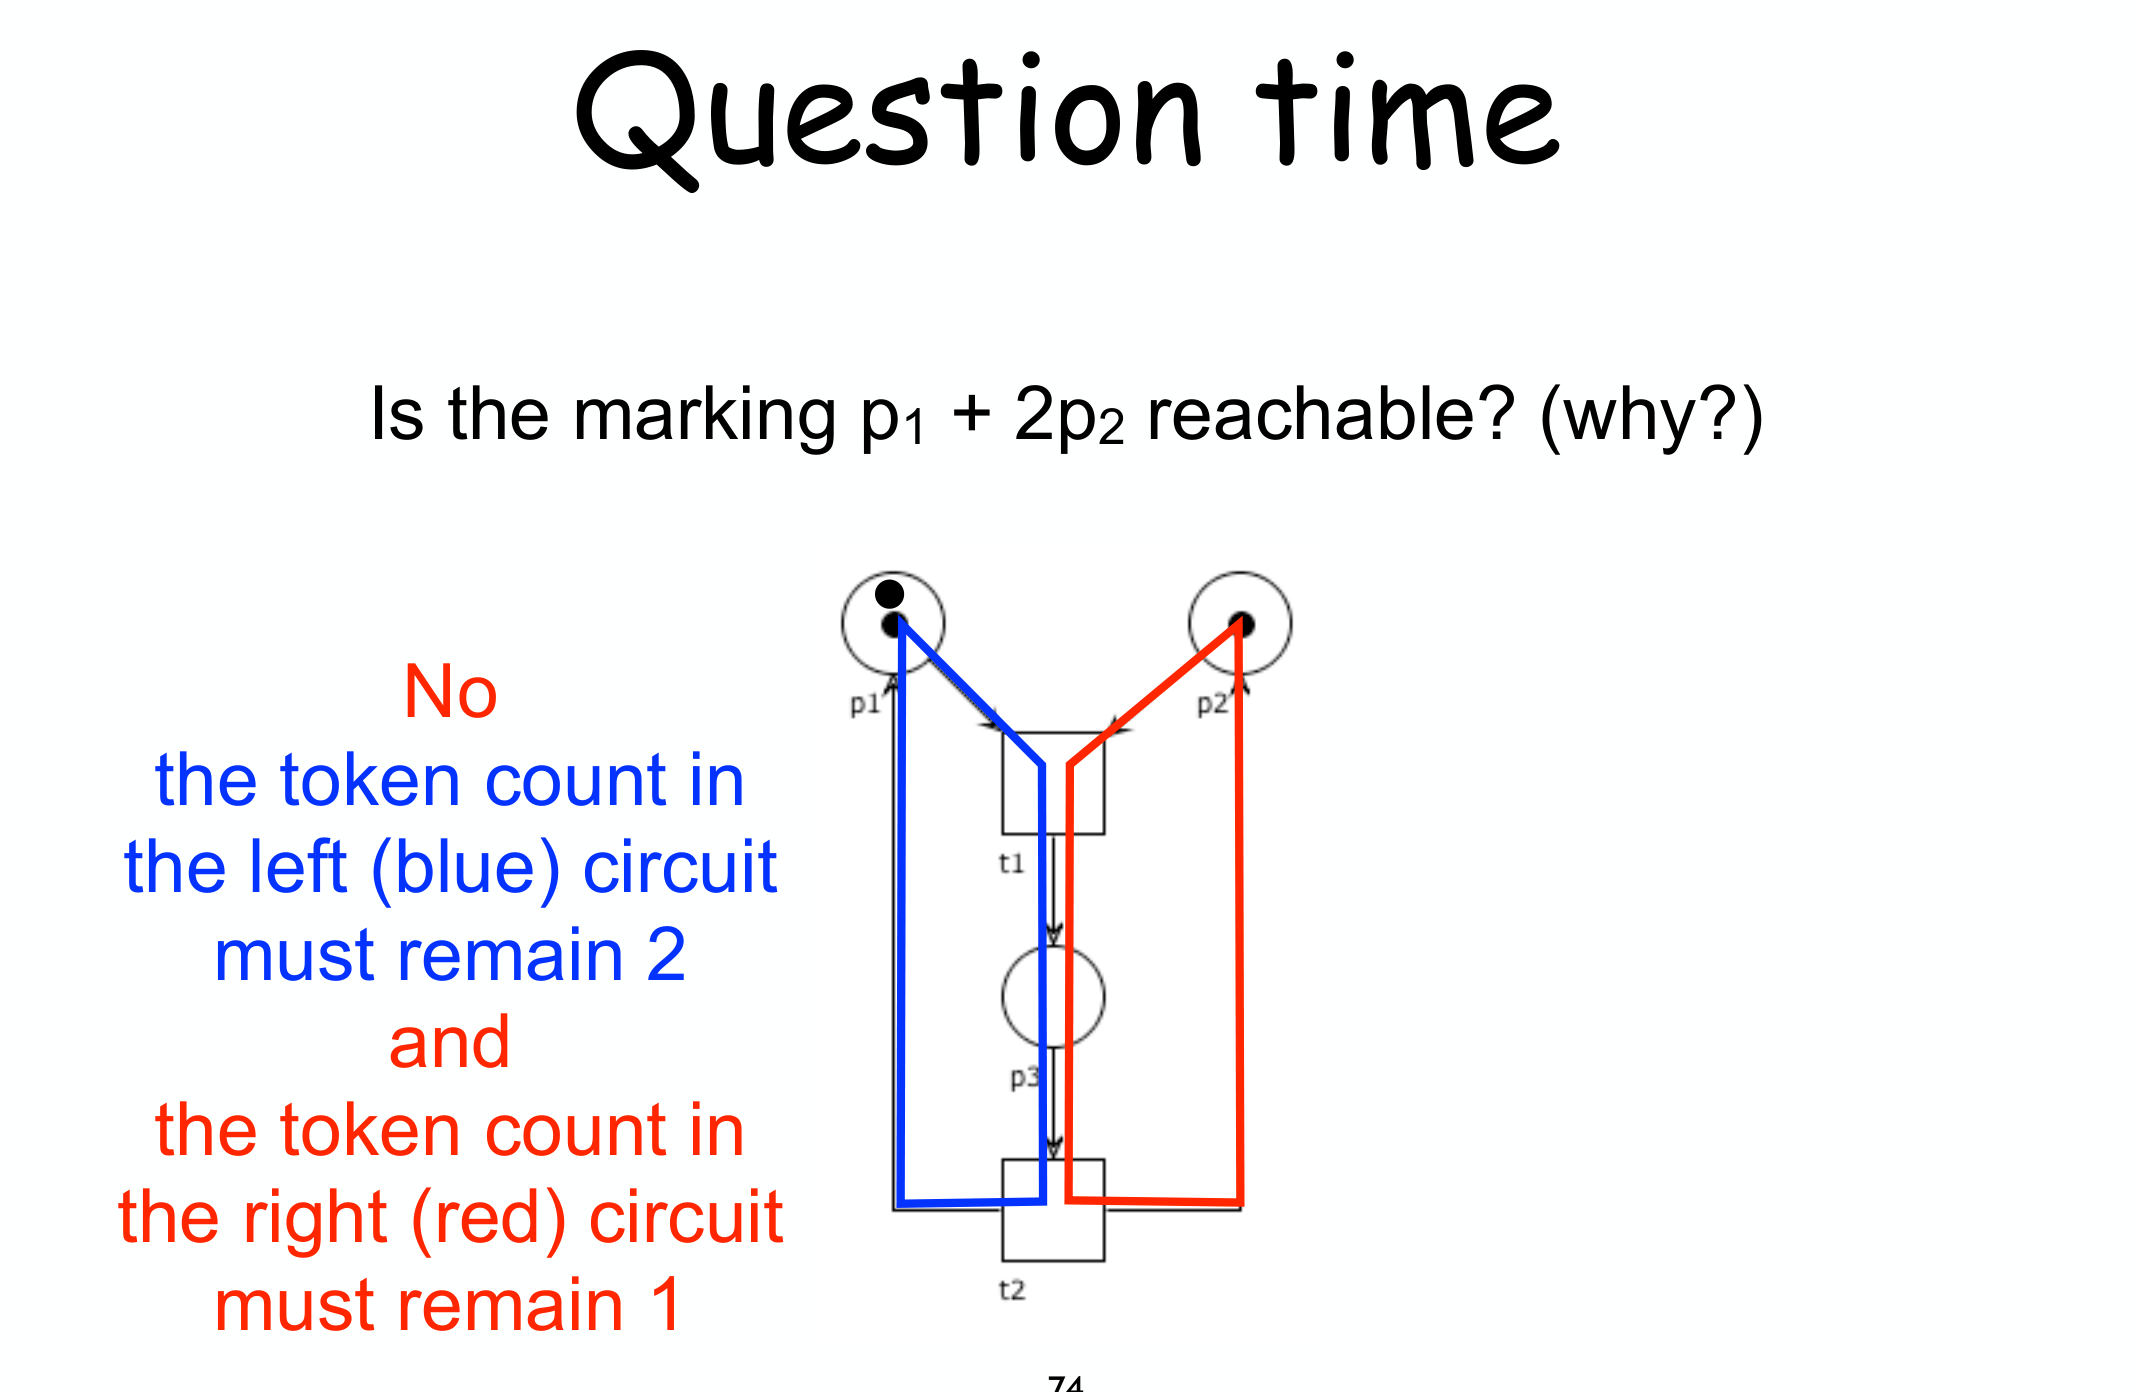
\includegraphics[width=0.74\linewidth,height=0.34\textheight,keepaspectratio]{images/15-st-systems_p73_circuit-reachability.png}
\caption{Usare i circuiti per la raggiungibilità. Ogni circuito ha un budget fisso di token: se la marcatura-obiettivo viola anche un solo budget (qui il circuito blu deve valere 2, il rosso 1), quella marcatura è irraggiungibile — senza costruire alcun reachability graph.}
\end{figure}

E la liveness dei T-system? Anch'essa strutturale, ed è forse il criterio più elegante della lezione.

\begin{boxtheorem}{Liveness dei T-system}
Un T-system $(N, M_0)$ è \textbf{live} $\iff$ \textbf{ogni circuito} di $N$ è \textbf{marcato} in $M_0$, cioè:

\[
M_0(\gamma) > 0 \quad \text{per ogni circuito } \gamma
\]

\emph{Intuizione ($\Rightarrow$ per assurdo):} se un circuito $\gamma$ ha zero token, per la proprietà fondamentale \textbf{resterà vuoto per sempre}; ma allora una transizione che ha un input place in $\gamma$ non riceverà mai un token da lì e non scatterà mai $\rightarrow$ è dead $\rightarrow$ non live. Viceversa, se ogni circuito ha almeno un token, si dimostra che ogni transizione può sempre essere riabilitata.
\end{boxtheorem}

\section{\texorpdfstring{Il quadro duale e le conseguenze sui workflow net}{Il quadro duale e le conseguenze sui workflow net}}

Le due teorie sono l'una lo specchio dell'altra. Vale la pena vederle affiancate.

\begin{boxabstract}{S-system vs T-system: la dualità}
\begingroup\small
\begin{tabularx}{\linewidth}{>{\raggedright\arraybackslash}X>{\raggedright\arraybackslash}X>{\raggedright\arraybackslash}X}
\toprule
\textbf{} & \textbf{\textbf{S-system}} & \textbf{\textbf{T-system}} \\
\midrule
Vincolo & ogni \textbf{transizione} 1-in-1-out & ogni \textbf{place} 1-in-1-out \\
Vieta & la \textbf{sincronizzazione} & la \textbf{scelta / conflitto} \\
Conservazione & token \textbf{totali} $M(P)$ & token per \textbf{circuito} $M(\gamma)$ \\
Sempre bounded? & \textbf{sì} (bounded da $M_0(P)$) & se \textbf{strongly connected} \\
Live $\iff$ & strongly connected + $M_0(P)\ge1$ & ogni circuito marcato \\
Invariante uniforme & S-invariant $[k\dots k]$ & T-invariant $[k\dots k]$ \\
\bottomrule
\end{tabularx}
\endgroup

La simmetria è perfetta scambiando \emph{place $\leftrightarrow$ transition}, \emph{token totali $\leftrightarrow$ token dei circuiti}, \emph{sincronizzazione $\leftrightarrow$ scelta}.
\end{boxabstract}

Il pagamento finale sono due criteri di \textbf{soundness verificabili a occhio} sui workflow net, senza alcuna analisi comportamentale.

\begin{boxtheorem}{Soundness strutturale dei workflow net}
\begin{itemize}
\item \textbf{Se un workflow net $N$ è un S-net, allora è safe e sound.} (Un solo caso che scorre, nessuna sincronizzazione: la correttezza è automatica.)
\item \textbf{Se un workflow net $N$ è tale che $N^\star$ è un T-net, allora $N$ è safe e sound $\iff$ ogni circuito di $N^\star$ è marcato.} (Nota: $N$ stesso non può essere un T-net, perché il place $i$ non ha input e $o$ non ha output; ma $N^\star$, con la transizione reset, può esserlo.)
\end{itemize}
\end{boxtheorem}

Questi due teoremi sono il coronamento del percorso sui Petri net: partiti dal disegno intuitivo, siamo arrivati a \textbf{certificare la correttezza di un processo controllando solo la struttura del grafo}. Nelle prossime lezioni torneremo alle notazioni di alto livello (EPC, BPMN) per applicarvi questi strumenti di analisi. $\rightarrow$ \hyperref[ch:16a]{16a — EPC Analysis}